
%(BEGIN_QUESTION)
% Copyright 2006, Tony R. Kuphaldt, released under the Creative Commons Attribution License (v 1.0)
% This means you may do almost anything with this work of mine, so long as you give me proper credit

The following storage vessel holds liquid heptane, a hydrocarbon with an approximate specific gravity of 0.68.  A pressure transmitter located at the bottom infers heptane level by hydrostatic pressure (head).  Determine the calibration range of this pressure transmitter in order to properly translate the range of vessel level (0 to 14 feet) into an output signal of 4 to 20 mA.  Please express the transmitter's calibration range in units of inches W.C. (inches of water column).

$$\includegraphics[width=15.5cm]{i00241x01.eps}$$

Then, determine the following (assuming the transmitter has been properly calibrated for the application):

\begin{itemize}
\item{} Transmitter output signal (mA) at 8 feet of level
\item{} Heptane level at 5.7 mA signal output
\end{itemize}

\underbar{file i00241}
%(END_QUESTION)





%(BEGIN_ANSWER)

Lower range-values (LRV): 0 inches W.C. input = 4 mA output

\vskip 10pt

Upper range-values (URV): 114.24 inches W.C. input = 20 mA output

\vskip 10pt

\begin{itemize}
\item{} Transmitter output signal (mA) at 8 feet of level = 13.14 mA
\item{} Heptane level at 5.7 mA signal output = 1.4875 feet
\end{itemize}

%(END_ANSWER)





%(BEGIN_NOTES)


%INDEX% Measurement, level: hydrostatic pressure

%(END_NOTES)


